\ifx\boi\undefined\ifx\problemname\undefined
\providecommand\sampleinputname{}
\providecommand\sampleoutputname{}
\documentclass[polish]{templates/boi}
\problemlanguage{.pl}
\fi
\newcommand{\boi}{Bałtycka Olimpiada Informatyczna}
\newcommand{\practicesession}{Dzień próbny}
\newcommand{\contestdates}{27 kwietnia - 1 maja 2018}
\newcommand{\dayone}{Dzień 1}
\newcommand{\daytwo}{Dzień 2}
\newcommand{\licensingtext}{To zadanie jest objęte licencją CC BY-SA 4.0.}
\newcommand{\problem}{Zadanie}
\newcommand{\inputsection}{Wejście}
\newcommand{\outputsection}{Wyjście}
\newcommand{\interactivity}{Interakcja}
\newcommand{\grading}{Ocenianie}
\newcommand{\scoring}{Punkty}
\newcommand{\constraints}{Ograniczenia}
\renewcommand{\sampleinputname}{Przykładowe wejście}
\renewcommand{\sampleoutputname}{Przykładowe wyjście}
\newcommand{\sampleexplanation}[1]{Wyjaśnienie do przykładu #1}
\newcommand{\sampleexplanations}{Wyjaśnienie do przykładów}
\newcommand{\timelimit}{Limit czasu}
\newcommand{\memorylimit}{Limit pamięci}
\newcommand{\seconds}{s}
\newcommand{\megabytes}{MB}
\newcommand{\group}{Grupa}
\newcommand{\points}{Punkty}
\newcommand{\limitsname}{Limity}
\newcommand{\additionalconstraints}{Dodatkowe ograniczenia}
\newcommand{\testgroups}{
Zestaw testów dzieli się na kilka grup, każda jest warta pewną liczbę punktów.
Każda grupa składa się z jednego bądź większej liczby testów.
Aby otrzymać punkty za daną grupę, Twoje rozwiązanie musi przejść wszystkie testy z tej grupy.
Ostateczny wynik za zadanie jest liczony jako maksymalny wynik z pojedynczych zgłoszeń.
}



% \fi
% \newcommand{\boi}{Baltic Olympiad in Informatics}
% \newcommand{\practicesession}{Practice Session}
% \newcommand{\contestdates}{April 27 - May 1, 2018}
% \newcommand{\dayone}{Day 1}
% \newcommand{\daytwo}{Day 2}
% \newcommand{\licensingtext}{This problem is licensed under CC BY-SA 4.0.}
% \newcommand{\problem}{Problem}
% \newcommand{\inputsection}{Input}
% \newcommand{\outputsection}{Output}
% \newcommand{\interactivity}{Interactivity}
% \newcommand{\grading}{Grading}
% \newcommand{\scoring}{Scoring}
% \newcommand{\constraints}{Constraints}
% \renewcommand{\sampleinputname}{Sample Input}
% \renewcommand{\sampleoutputname}{Sample Output}
% \newcommand{\sampleexplanation}[1]{Explanation of Sample #1}
% \newcommand{\sampleexplanations}{Explanation of Samples}
% \newcommand{\timelimit}{Time Limit}
% \newcommand{\memorylimit}{Memory Limit}
% \newcommand{\seconds}{s}
% \newcommand{\megabytes}{MB}
% \newcommand{\group}{Group}
% \newcommand{\points}{Points}
% \newcommand{\limitsname}{Limits}
% \newcommand{\additionalconstraints}{Additional Constraints}
% \newcommand{\testgroups}{
% Your solution will be tested on a set of test groups, each worth a number of points.
% Each test group contains a set of test cases.
% To get the points for a test group you need to solve all test cases in the test group.
% }
\fi
\def\version{jury-1}
\problemname{Ścieżki}
{\em Graf} to struktura matematyczna złożona ze zbioru {\em wierzchołków} i zbioru {\em krawędzi}, każda krawędź
łączy dwa wierzchołki. Przykładowy graf o $4$ wierzchołkach i $3$ krawędziach jest pokazany w wyjaśnieniu pierwszego testu przykładowego.

{\em Ścieżka} to ciąg $2$ lub więcej wierzchołków taki, że każde dwa kolejne wierzchołki w ciągu są połączone krawędzią. W tym zadaniu będziemy rozważali {\em prote ścieżki}, to jest takie, w których żaden wierzchołek nie występuje więcej niż raz.
Kolejność wierzchołków ma znaczenie; przykładowo ,,\texttt{5-6-7}'', ,,\texttt{5-7-6}'' and ,,\texttt{7-6-5}'' to różne ścieżki.


Każdy wierzchołek ma jeden z $K$ kolorów. Twoim zadaniem jest znalezienie liczby różnych (prostych) ścieżek,
na~których wszystkie wierzchołki mają różne kolory.


\section*{\inputsection}
Pierwszy wiersz wejścia zawiera trzy liczby całkowite: $N$ (liczbę wierzchołków), $M$ (liczbę krawędzi) i $K$ (liczbę kolorów).

%($1 \le N, M \le 3 \cdot 10^5, 1 \le K \le 5$).

Drugi wiersz wejścia zawiera $N$ liczb całkowitych pomiędzy $1$ a $K$ -- kolory wierzchołków (kolejno dla wierzchołków od $1$ do $N$).

Każdy z kolejnych $M$ wierszy opisuje krawędź i zawiera dwie liczby całkowite $a, b$ ($1 \le a, b \le N, a \neq b$) -- numery
wierzchołków połączonych krawędzią. Między każdą parą wierzchołków będzie co najwyżej jedna krawędź.

\section*{\outputsection}
Na wyjście wypisz pojedynczą liczbę całkowitą -- liczbę ścieżek, na których wszystkie wierzchołki mają parami różne kolory.
Wynik nie przekroczy $10^{18}$.

\section*{\constraints}
\testgroups

\noindent
\begin{tabular}{| l | l | l |}
\hline
\group & \points & \limitsname \\ \hline
1      & 23      & $1 \le N, M \le 100, 1 \le K \le 4$ \\ \hline
2      & 20      & $1 \le N, M \le 300\,000, 1 \le K \le 3$ \\ \hline
3      & 27      & $1 \le N, M \le 300\,000, 1 \le K \le 4$ \\ \hline
4      & 30      & $1 \le N, M \le 100\,000, 1 \le K \le 5$ \\ \hline
\end{tabular}

\section*{\sampleexplanation{1}}

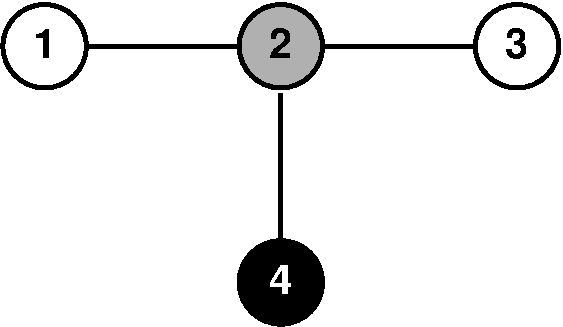
\includegraphics[width=5cm]{pathsfig.pdf}

Rysunek przedstawia graf z pierwszego testu przykładowego, każdy wierzchołek ma kolor biały (kolor 1), szary (kolor 2) lub czarny (kolor 3).
Jest 10 ścieżek, na których wszystkie wierzchołki mają różne kolory:
,,\texttt{1-2}'', ,,\texttt{2-1}'', ,,\texttt{2-3}'', ,,\texttt{3-2}'', ,,\texttt{2-4}'', ,,\texttt{4-2}'', ,,\texttt{1-2-4}'', ,,\texttt{4-2-1}'', ,,\texttt{3-2-4}'' oraz ,,\texttt{4-2-3}''.

,,\texttt{1}'' nie jest poprawną ścieżką, ponieważ zawiera tylko jeden wierzchołek, jak również
,,\texttt{1-2-3}'', ponieważ zawiera dwa wierzchołki o kolorze $1$.
